\chapter{template}

\section{Cross reference} \label{template_cross_reference}

The code snippet for list is given Section~\ref{template_list}.
The \texttt{~} makes sure three is a space between Section and the reference number but no new line split between them.



\section{Lists} \label{template_list}

\subsection{Bullet points}
\begin{itemize}
  \item Fish
  \item Animals
  \begin{itemize}
    \item Domesticated animals
    \begin{itemize}
      \item Cow
    \end{itemize}
  \end{itemize}
\end{itemize}

\subsection{Numbered list}

\begin{enumerate}
  \item Fish
  \item Animals
  \begin{enumerate}
    \item Domesticated animals
    \begin{enumerate}
      \item Cow
    \end{enumerate}
  \end{enumerate}
\end{enumerate}

\section{Code section}
\texttt{minted} package includes formated code sections.
The code section can be embedded or from a file.

\texttt{listing} package includes code sections with caption and lable.
But it does not supporet formated code or code section from a file.

So combining \texttt{minted} and \texttt{listing} gives us nice formated code section.


\begin{listing}[!ht]
\usemintedstyle{vim}
\begin{minted}[linenos]{bash}
  export PAGER=~/source/vimpager/vimpager
  alias less=$PAGER
  alias zless=$PAGER
  set -o vi
  export EDITOR=vim
  alias trim='~/bin/trim.sh'
  alias ctag='ctags -L .files.txt --c-kinds=+px'
  alias inkscape='UBUNTU_MENUPROXY=0 inkscape'

  if [[ -f ~/.git-completion.bash ]]; then
  source ~/.git-completion.bash
  source ~/.git-prompt.sh
  source /usr/share/bash-completion/completions/git
  fi

  #export PS1="\[\e[1;32m\e[40m\]\h \[\e[m\]|\W: "
  #export PS1="$"
\end{minted}
\caption{embedded bash script}
\label{embedded_code_section}
\end{listing}

\begin{listing}[!ht]
\usemintedstyle{vim}
  \inputminted[linenos]{cpp}{template/source/helloWorld.cpp}
\caption{C++ code from a file}
\label{file_code_section}
\end{listing}

\section{Figures}%
\label{sub:figures}

Figure~\ref{fig:Example} is an example figure.


\begin{figure}[h]
\caption{An example figure}
\centering
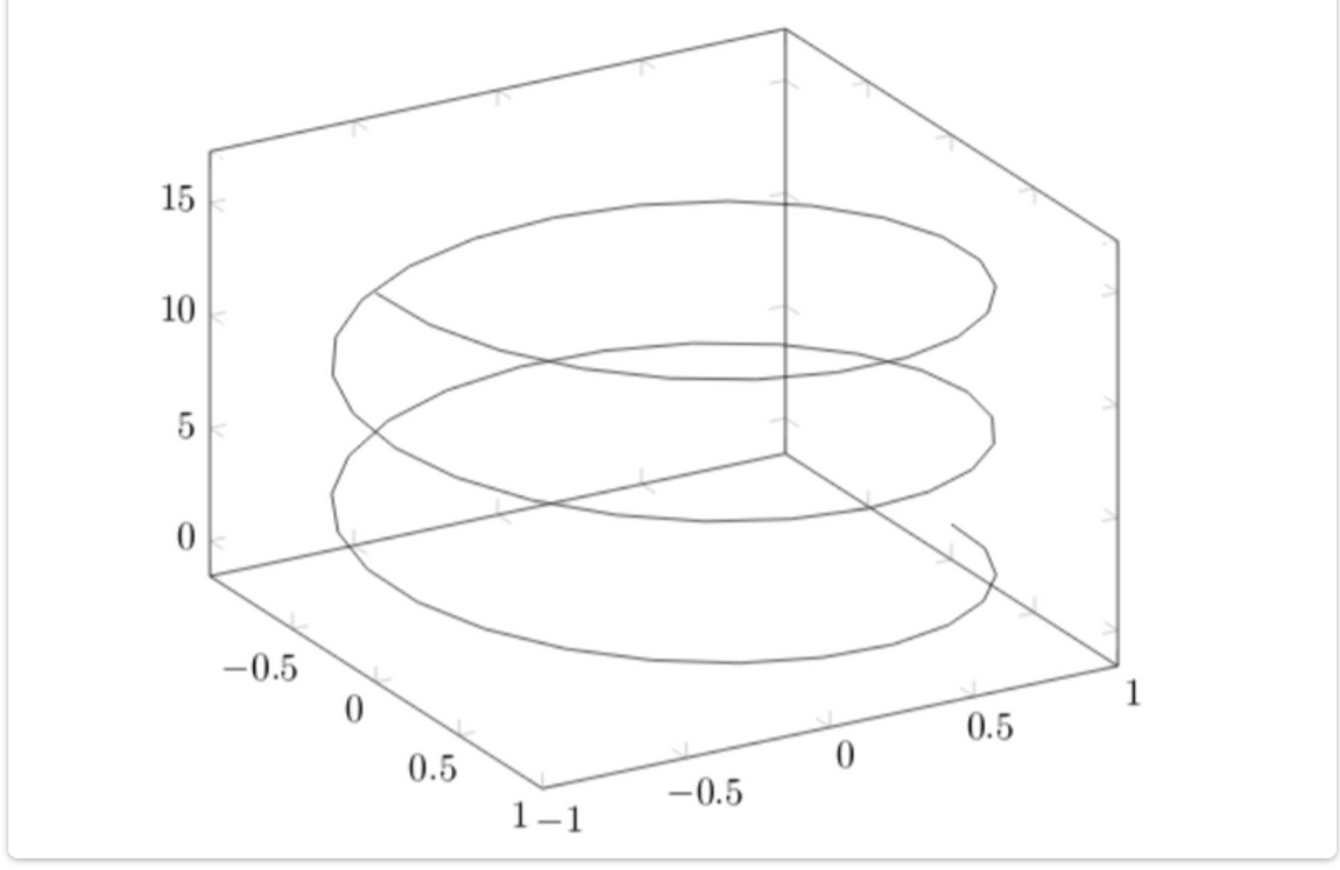
\includegraphics[width=0.5\textwidth]{./template/figure.pdf}
\label{fig:Example}
\end{figure}

\section{Reference}

\begin{enumerate}
  \item \href{https://www.google.com/}{google}
  \item \href{https://www.google.com/}{google}
\end{enumerate}

\section{Markdown in latex}%
\label{sec:markdown_in_latex}
Markdown files can be included in latex. \\


\markdownInput{template/source/README.md}

Or Markdown code can be included in latex. \\

\begin{markdown}
### An h3 header

Paragraphs are separated by a blank line.

2nd paragraph. *Italic*, **bold**, and `monospace`. Itemized lists
look like:

* this one
* that one
* the other one

> Block quotes are
> written like so.
>
> They can span multiple paragraphs,
> if you like.

\end{markdown}
